\documentclass[fleqn]{article}
\usepackage[utf8]{inputenc}

\title{Compte rendu\\ Projet de Calcul Scientifique Numérique \\ Etude de la réponse d'un thermocouple par la méthode des différences finies} 
\author{Belpois Vincent \\ Chomette Hugo}
\date{}
\usepackage[fleqn]{mathtools}
\usepackage{amssymb}
\usepackage{enumitem}
\usepackage{amsfonts}
\usepackage{amsmath}
\usepackage{geometry}
\usepackage{graphicx}
\usepackage{xcolor}
\usepackage{esint}          % various fancy integral symbols
\usepackage{upgreek}
\usepackage{parskip}
\usepackage[b]{esvect}      %For better vectors
\usepackage{float}
\usepackage{tikz}
\usepackage{pdflscape}

\usepackage{pythonhighlight}

\usepackage[loop, autoplay, controls = all]{animate}

\usepackage{hyperref}
\hypersetup{
    colorlinks,
    citecolor=black,
    filecolor=black,
    linkcolor=black,
    urlcolor=black
}


\geometry{hmargin=2.5cm,vmargin=1.5cm}

\usepackage{sectsty}

\renewcommand*\contentsname{Table des matières}

\renewcommand{\epsilon}{\varepsilon} 
\renewcommand{\phi}{\varphi} 
\newcommand{\dd}{\text{d}}

\let\vect\overrightarrow
\let\mc\mathcal




\setlist[1]{noitemsep}



\begin{document}
\maketitle

\begin{figure}[H]
    \centering
    \includegraphics[width = 0.5\paperwidth]{images/Page de garde.png}
\end{figure}
\vspace{10pt}
\begin{figure}[H]
    \centering
    \includegraphics[width = 0.25\paperwidth]{images/Logo_ISAE-ENSMA.svg.png}
\end{figure}


\newpage

\tableofcontents
\newpage

\section{Présentation du problème}
\subsection{Le problème}
On modélise un thermocouple par une sphère uniforme de rayon $a$. Cette sphère, initialement à la température $T_0$, échange convectivement avec le milieu extérieur, à la température $T_\infty$, selon la loi $\phi = h(\theta) ( T - T_\infty)$. 
\begin{figure}[H]
    \centering
    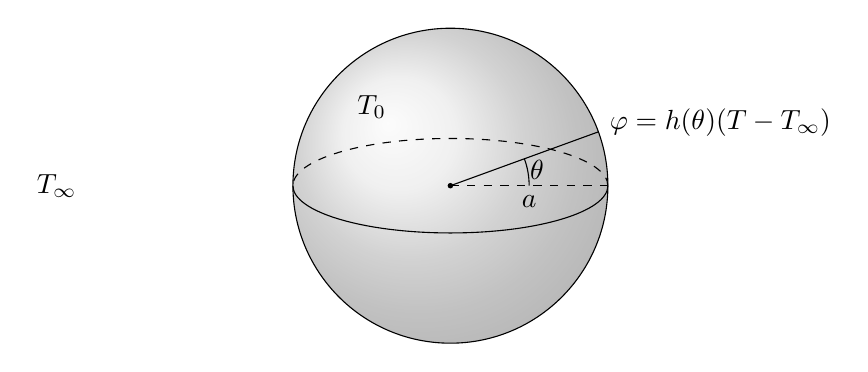
\begin{tikzpicture}
        \shade[ball color = gray!40, opacity = 0.4] (0,0) circle (2cm);
        \draw (0,0) circle (2cm);
        \draw (-2,0) arc (180:360:2 and 0.6);
        \draw[dashed] (2,0) arc (0:180:2 and 0.6);
        \fill[fill=black] (0,0) circle (1pt);
        \draw[dashed] (0,0 ) -- node[below]{$a$} (2,0);
        \draw (0,0) -- ({2*cos(20)},{2*sin(20)});
        \draw (1,0) arc (0:20:1);
        \node at (1.1,0.2) {$\theta$};
        \node at (1.9,0.8) [right]{$\phi = h(\theta) ( T - T_\infty)$};
        \node at (-5, 0) {$T_\infty$};
        \node at (-1,1) {$T_0$};
    \end{tikzpicture}
    \caption{Schéma du thermocouple}
\end{figure}


On cherche alors à étudier la réponse de ce thermocouple au cours du temps. Pour cela, on s'impose l'utilisation de la méthode des différences finies.


\subsection{Interprétation des coefficients}
La fonction $h(\theta)$ décrit la dépendance de la convection avec l'angle $\theta$ entre la normale à la surface de la sphère et la direction de l'échange thermique. Plus précisément, la quantité de chaleur échangée par convection entre la sphère et le milieu extérieur est proportionnelle à la différence de température entre la sphère et le milieu extérieur, multipliée par $h(\theta)$.

La forme de la fonction $h(\theta) = K (1 + \cos(\theta))$ indique que l'échange de chaleur par convection est maximal lorsque la normale à la surface de la sphère est parallèle à la direction de l'échange thermique et dans le même sens que celui-ci, c'est-à-dire lorsque $\theta = 0^\circ$. Dans ces cas, $h(\theta) = K (1 + 1) = 2K$. L'échange de chaleur par convection est minimal lorsque la normale à la surface de la sphère est dans le sens opposé à celui de l'échange thermique, c'est-à-dire lorsque $\theta = 180^\circ$. Dans ce cas, $h(\theta) = K (1 - 1) = 0$.

La constante $K$ détermine l'intensité de l'échange de chaleur par convection pour un angle $\theta$ donné. Plus $K$ est grand, plus l'échange de chaleur par convection est important. $K$ est alors exprimé en $W.m^{-2}.K^{-1}$, tout comme $h(\theta)$.

\subsection{Mise en équation du problème}
Ce problème revient alors à résoudre l'équation de la chaleur en 3 dimensions et au cours du temps.
De manière générale, l'équation de la chaleur s'écrit de la manière suivante :
\begin{equation}
    \rho C_p \left(  \frac{ \partial T}{\partial t} + u \cdot \nabla T \right) = \nabla \cdot ( \lambda  \nabla T) + s
\end{equation}

Dans notre cas, cette équation peut être simplifiée. On a premièrement $u = 0$ car la sphère n'est pas en mouvement. De plus, lambda est constant, on a donc, par linéarité du gradient, $\nabla ( \lambda \nabla T ) = \lambda \nabla^2 T$. Enfin, le thermocouple n'étant traversé par aucun courant électrique, aucune chaleur n'est produite en son sein et donc le terme de source $s$ est nul.

L'équation de la chaleur devient alors :
\begin{equation}
    \rho C_p   \frac{ \partial T}{\partial t} = \lambda\nabla^2 T
    \label{equation_de_la_chaleur}
\end{equation}

On peut aussi écrire une condition à la surface de la sphère, représentant un échange convectif :
\[
\phi = h(\theta)(T-T_\infty)
\] 
Avec $h(\theta)$ le coefficient de convection exprimé précédemment.


\newpage
\section{Choix du système de coordonnées et du maillage}
\subsection{Comparaison des systèmes de coordonnées cartésiennes et sphériques}
\subsubsection{Coordonnées cartésiennes}
Le système de coordonnées cartésiennes a l'avantage d'utiliser un repère orthonormé. L'expression des opérateurs tels que le laplacien est donc simple et les équations sont alors simplifiées. Cependant, si le maillage n'est pas régulier selon les trois axes du système de coordonnées cartésiennes, l'expression du pas est alors plus complexe.

\begin{figure}[H]
    \centering
    \includegraphics[width = 0.3\paperwidth]{images/Rectangular_coordinates.svg.png}
    \caption{Repère cartésien}
\end{figure}

\subsubsection{Coordonnées sphériques}
Le problème décrivant une sphère, le seul système de coordonnées qui peut-être intéressant à utiliser est le système de coordonnées sphériques. Ce système de coordonnées est aussi constitué de trois axes orthonormés:$\vv{e_r}, \vv{e_\theta}, \vv{e_\phi}$ . On utilisera alors pour décrire la position d'un point un triplet de coordonnées $(r, \theta, \phi)$. 

\begin{figure}[H]
    \centering
    \includegraphics[width = 0.3\paperwidth]{images/Spherical_Coordinates.png}
    \caption{Repère sphèrique}
\end{figure}


Pour passer des coordonnées cartésiennes aux coordonnées sphériques on utilise les équations suivantes :
\begin{equation}
    \begin{cases}
        r = \sqrt{x^2 + y^2 + z^2} \\
        \theta = \arccos \left( \frac{z}{r} \right)\\
        \phi = \arctan \left( \frac{y}{x} \right)
    \end{cases}
\end{equation}

De la même manière, pour passer des coordonnées sphériques aux coordonnées cartésiennes on utilise les équations suivantes :
\begin{equation}
    \begin{cases}
        x&=r \sin \theta \cos \varphi \\
        y&=r \sin \theta \sin \varphi \\
        z&=r \cos \theta 
    \end{cases}
    \label{Polar coord}
\end{equation}

\subsection{Réécriture des équations adaptée au nouveau système de coordonnées}
 
L'équation de la chaleur Eq.\eqref{equation_de_la_chaleur} utilise l'opérateur laplacien ($\Delta = \nabla^2$). Cet opérateur s'écrit en coordonnées cartésiennes :

\begin{equation}
    \Delta f = {\frac {\partial ^{2}f }{\partial x^{2}}}+{\frac {\partial ^{2}f }{\partial y^{2}}}+{\frac {\partial ^{2}f }{\partial z^{2}}}
\end{equation}

En coordonnées sphériques, cet opérateur s'écrit alors :
\begin{equation}
     \Delta f={\frac {\partial ^{2}f}{\partial r^{2}}}+{\frac {1}{r}}{\frac {\partial f}{\partial r}}+{\frac {1}{r^{2}}}{\frac {\partial ^{2}f}{\partial \theta ^{2}}}+{\frac {1}{r^{2}\tan \theta }}{\frac {\partial f}{\partial \theta }}+{\frac {1}{r^{2}\sin ^{2}\theta }}{\frac {\partial ^{2}f}{\partial \varphi ^{2}}}
\end{equation}

L'équation de la chaleur Eq.\eqref{equation_de_la_chaleur} s'écrit alors :
\begin{equation}
    \rho C_p \frac{ \partial T}{\partial t}  = \lambda \left( 
    {\frac {\partial ^{2}T}{\partial r^{2}}}+{\frac {1}{r}}{\frac {\partial T}{\partial r}}+{\frac {1}{r^{2}}}{\frac {\partial ^{2}T}{\partial \theta ^{2}}}+{\frac {1}{r^{2}\tan \theta }}{\frac {\partial T}{\partial \theta }}+{\frac {1}{r^{2}\sin ^{2}\theta }}{\frac {\partial ^{2}T}{\partial \varphi ^{2}}} \right)      
\end{equation}
Dans la suite du problème on utilisera la constante $\alpha = \frac{\lambda}{\rho C_p}$ afin de simplifier l'écriture de l'équation ci-dessus.

\subsection{Maillage de la sphère}
Une sphère peut être maillée de plusieurs manières dans un espace 3D, certains maillages favoriseront l'uniformité de la taille des mailles comme les maillages quadrangulaires ou en géode par triangulation tandis que d'autres faciliteront la résolution numérique du problème comme le maillage en sphère UV (maillage en faces rectangulaires, formé par des segments assimilables à des lignes de longitude et de latitude sur un globe).
\begin{center}
    \begin{minipage}[b]{0.33333\textwidth}
        \begin{figure}[H]
            \centering
            \includegraphics[width = 0.5\textwidth]{images/sphere quad.png}
            \caption{Sphère quadrangulaire}
        \end{figure}
    \end{minipage}
    \begin{minipage}[b]{0.33333\textwidth}
    \centering
    \begin{figure}[H]
        \centering
        \includegraphics[width = 0.5\textwidth]{images/sphere iso.png}
        \caption[short]{Sphère ISO ou en géode}
    \end{figure}
    \end{minipage}%
    \begin{minipage}[b]{0.33333\textwidth}
    \begin{figure}[H]
        \centering
        \includegraphics[width = 0.5\textwidth]{images/sphere UV.png}
        \caption[short]{Sphère UV}
    \end{figure}
    \end{minipage}
\end{center}


On utilisera dans le cadre de notre simulation un maillage UV de la sphère, ce modèle se prêtant très bien au système de coordonnées sphériques. Cela simplifiera les calculs et l'implémentation des équations.

Les paramètres pour construire ce maillage seront alors \texttt{Nr, Ntheta, Nphi}, représentant respectivement le nombre de mailles dans la direction $r$, la direction $\theta$, et la direction $\phi$ 

On repèrera par le triplet $(i,j,k)$ les coordonnées du noeud du maillage de la sphère. 

\newpage
\section{Discrétisation du problème} 
La méthode utilisée ici est la méthode des différences finies. On choisit d'utiliser l'ordre 1 afin de simplifier les expressions des termes de l'équation de la chaleur, un ordre supérieur pourra être utilisé afin d'augmenter la précision et la stabilité si nécessaire.
\subsection{Discrétisation de l'équation de la chaleur}
On rapelle l'équation de la chaleur utilisée :

\begin{equation}
    \frac{ \partial T}{\partial t}  =  \alpha \nabla^2 T
\end{equation}

Et donc en coordonnées sphériques, en prenant en compte l'invariance du champ de température par rapport à $\phi$  :

\begin{equation}
    \frac{ \partial T}{\partial t}  = \alpha \left( 
    {\frac {\partial ^{2}T}{\partial r^{2}}}+{\frac {1}{r}}{\frac {\partial T}{\partial r}}+{\frac {1}{r^{2}}}{\frac {\partial ^{2}T}{\partial \theta ^{2}}}+{\frac {1}{r^{2}\tan \theta }}{\frac {\partial T}{\partial \theta }} \right)      
\end{equation}

On cherche à exprimer $T^n $ en fonction uniquement de $T^{n-1}$ On utilise alors un schéma arrière temporel. : 

\begin{equation}
    \frac{ \partial T}{\partial t} \rightarrow  \frac{T^n - T^{n-1}}{\Delta t} 
\end{equation}

On discrétise ensuite avec un schéma centré les termes issus du laplacien de la température :


\begin{equation}
    \frac{ \partial ^2 T}{\partial r^2} \rightarrow 
    \frac{T_{i+1,j,k}^{n-1} - 2 T_{i,j,k}^{n-1} + T_{i-1,j,k}^{n-1}}{\Delta r^2}
\end{equation}

\begin{equation}
    \frac{1}{r}\frac{ \partial T}{\partial r} \rightarrow 
    \frac{1}{r_i}\frac{T_{i+1,j,k}^{n-1} - T_{i-1,j,k}^{n-1}}{\Delta r}
\end{equation}

\begin{equation}
    \frac{1}{r^2}\frac{ \partial^2 T}{\partial \theta^2} \rightarrow 
    \frac{1}{r_i^2}\frac{T_{i,j+1,k}^{n-1} - 2 T_{i,j,k}^{n-1} + T_{i,j-1,k}^{n-1}}{\Delta \theta^2}
\end{equation}

\begin{equation}
    \frac{1}{r^2 \tan \theta}\frac{ \partial T}{\partial \theta} \rightarrow 
    \frac{1}{r_i^2 \tan \theta_j }\frac{T_{i,j+1,k}^{n-1} - T_{i,j-1,k}^{n-1}}{2\Delta \theta}
\end{equation}


On peut alors exprimer $T^n$ :

\begin{multline}
    T^n = \alpha \Delta t  \left( \frac{T_{i+1,j,k}^{n-1} - 2 T_{i,j,k}^{n-1} + T_{i-1,j,k}^{n-1}}{\Delta r^2}+\frac{1}{r_i}\frac{T_{i+1,j,k}^{n-1} - T_{i-1,j,k}^{n-1}}{\Delta r} + \frac{1}{r_i^2}\frac{T_{i,j+1,k}^{n-1} - 2 T_{i,j,k}^{n-1} + T_{i,j-1,k}^{n-1}}{\Delta \theta^2}\right. \\
    +\left.\frac{1}{r_i^2 \tan \theta_j }\frac{T_{i,j+1,k}^{n-1} - T_{i,j-1,k}^{n-1}}{2\Delta \theta}\right)  + T^{n-1}
    \label{discretisation Gal}
\end{multline}


\subsection{Discrétisation des conditions aux limites}

On doit par la suite discrétiser notre condition à la surface de la sphère que l'on rappelle être :
\begin{equation}
    \phi = h(\theta)(T - T_{\infty})
\end{equation}

On a donc par la loi de Fourier :
\begin{equation}
    h(\theta)(T(r = a) - T_\infty) = -\lambda \left.\frac{ \partial T}{\partial r}\right|_{r=a} 
\end{equation}
On a alors, par les discrétisations des dérivées partielles précédentes :
\begin{equation}
    T_{i,j,k}^n = \left(h(\theta) + \frac{\lambda}{\Delta r}\right)^{-1} \cdot \left( h(\theta) T_\infty + \lambda \frac{T_{i-1,j,k}}{\Delta r}\right)
    \label{discretisation limite}
\end{equation}

Les équations Eq.\eqref{discretisation Gal}et Eq.\eqref{discretisation limite} nous permettent alors d'exprimer, en tout point de la sphère, la température en fonction des températures de la sphère à l'instant précédent





\section{Simulation Python} 
Pour implémenter une telle simulation, nous avons utilisé Python comme language de programmation pour sa facilité et sa capacité à visualiser des données à l'aide de bibliothèques simples. La capacité à exécuter du code sans compiler nous a aussi permis d'itérer plus rapidement et de débugger simplement le code.
\subsection{Structure du code}
Le code est composé de quelques fonctions simples et notre situation ne semblait pas demander à introduire de la programmation orientée objet, car nous avons décidé de représenter les maillages et les simulations commme de simples tableaux \texttt{numpy}. 

Ainsi, on commence d'abord par fixer nos constantes de la simulation comme les paramètres de maille, les constantes du matériau considéré, les températures ($T_0$ et $T_\infty$ ), le facteur de convection, etc\dots

On construit ensuite le maillage de la sphère.

Enfin on itère la simulation en stockant chaque maillage de la simulation dans une liste.

Finalement, on affiche cette simulation et on enregistre une animation de celle-ci.

\subsection{Implémentation du maillage}
 \subsubsection{Maillage et liste de maillages}
Chaque maillage de la sphère est représenté par un tableau \texttt{numpyarray} de dimension 4. Les 3 premières coordonnées sont utilisées pour la position (soit $x,y,z$ soit $r, \theta, \phi$ ) tandis que la quatrième est utilisée pour représenter la température de ce noeud. Ainsi, on crée un objet \texttt{maillage} de la manière suivante :


\begin{python}
    maillage = np.zeros((Nr,Ntheta,Nphi,4))
    maillage[:,:,:,3] = T0                  #initialise la temperature de chaque noeud a T_0
    for i in range(Nr):
        for j in range(Ntheta):
            for k in range(Nphi):
                maillage[i,j,k,:3] = ((i)*a/(Nr), (j+0.5)*math.pi/Ntheta, 2*k*math.pi/Nphi)

\end{python}
Les coordonnées sont alors données par Eq.\eqref{Polar coord}. On initialise tous les noeuds à la température $T_0$, température initiale du thermocouple supposé uniforme. 

On introduit aussi une fonction permettant d'obtenir le maillage constitué des coordonnées cartésiennes de chaque noeud afin de pouvoir visualiser ce maillage par la suite :
\begin{python}
    def polar_to_cartesian(polar):
        cart = np.copy(polar)
        cart[:,:,:,0] = polar[:,:,:,0] * np.sin(polar[:,:,:,1])*np.cos(polar[:,:,:,2])
        cart[:,:,:,1] = polar[:,:,:,0] * np.sin(polar[:,:,:,1])*np.sin(polar[:,:,:,2])
        cart[:,:,:,2] = polar[:,:,:,0] * np.cos(polar[:,:,:,1])
        return cart
\end{python}

On construit alors une simulation comme étant une liste de différents maillages (les maillages sont physiquement identiques mais la valeur de la température à chaque noeud est différente).
Cela peut se voir dans la fonction \texttt{simulation} qui ajoute à la liste de maillages, le nouveau maillage calculé par la fonction \texttt{compute\_next\_step}:

\begin{python}
    def simulation():
    dt = 0.000001
    meshes = []
    meshes.append(maillage)
    for i in range(25000):
        print(i)
        meshes.append(compute_next_step(meshes[i], dt))
    return meshes
\end{python}

\texttt{meshes} est alors l'ensemble des maillages de notre simulation.

\subsubsection{Visualisation des maillages et des simulations}
On a décidé d'utiliser la librairie \texttt{matplotlib} afin de visualiser nos données car cette librairie peut à la fois permettre de réaliser des visualisations 3D et de simples graphes 2D.

\begin{python}
    from mpl_toolkits.mplot3d import Axes3D
    import matplotlib.animation

    fig = plt.figure()
    fig.set_figheight(15)
    fig.set_figwidth(15)
    ax = fig.add_subplot(111, projection='3d')

    ax.axes.set_xlim3d(left=-0.004, right=0.004) 
    ax.axes.set_ylim3d(bottom=-0.004, top=0.004)
    ax.axes.set_zlim3d(bottom=-0.004, top=0.004)

    norm = matplotlib.colors.Normalize(vmin=380, vmax=451)
\end{python}

On commence par initialiser une figure avec une projection de type '3d'. On fixe alors les limites de l'affichage. Et enfin, on crée la variable \texttt{norm} qui sera utilisée lors de l'affichage des températures par une plage de couleurs.

On doit alors, pour afficher une animation des points qui changent de couleur au cours du temps, créer une fonction qui met à jour la visualisation, et change les données envoyées à \texttt{matplotlib} :
\begin{python}
    def update_graph(num):
        factor = 100
        global k
        mesh_c = polar_to_cartesian((simulation_meshes[num*factor]))
        graph._offsets3d = mesh_c[:,:,:,0].ravel(), mesh_c[:,:,:,1].ravel(), mesh_c[:,:,:,2].ravel()
        
        graph.set_facecolor(cmap_inferno(norm(mesh_c[:,:,:,3].ravel())))
            
        title.set_text('3D Test, num={}'.format(num*factor))
        return title, graph, 
\end{python}

Le paramètre \texttt{factor} est utilisé pour n'afficher que certaines étapes de la simulation, ici toutes les 100 mises à jours du maillage. Dans le cas contraire, la visualisation de l'entièreté de la simulation prendrait des heures.

On peut alors afficher la simulation de la manière suivante :
\begin{python}
    mesh_c = polar_to_cartesian((simulation_meshes[0]))
    graph = ax.scatter(mesh_c[:,:,:,0].ravel(), mesh_c[:,:,:,1].ravel(), mesh_c[:,:,:,2].ravel())
    ani = matplotlib.animation.FuncAnimation(fig, update_graph,249, blit=False)

    plt.show()
    ani.save("simulation.gif", fps=10)
\end{python}

Ici, 249 représente la dernière itération de la simulation que l'on souhaite voir (qui sera multiplié par \texttt{factor} et donc représente ici l'itération 24900). On sauvegarde aussi l'animation créée pour de prochaines visualisations.


\subsection{Implémentation des équations}
Les équations discutées dans les parties précédentes sont implémentées dans la fonction \texttt{compute\_next\_step}. Cette fonction prend en paramètre le maillage au temps $n$ et le pas temporel \texttt{dt} et renvoie le nouveau maillage au temps $n+1$.

Dans l'extrait de code qui suit, certaines parties ont été omises afin d'en faciliter la lecture. En effet on remarque que plusieurs cas selon la valeur de \texttt{i} ont été dissociés. Cela est dû au fait que l'expression du laplacien en différente en 0 et la présence de la condition à la surface de la sphère (en $r=a$). On remarque aussi que des distinctions de cas ont été faites selon la valeur de \texttt{j}. Cela provient des problèmes d'indices ; les indices ne forment pas une boucle lorsque l'on atteint le dernier indice.

\begin{python}
def compute_next_step(p_mesh, dt):
    Nr, Ntheta, Nphi, _ = np.shape(p_mesh)
    n_mesh = np.copy(p_mesh)

    Delta_r = a / Nr
    Delta_theta = math.pi / Ntheta
    Delta_phi = 2 * math.pi / Nphi
    for i in range(0, Nr):
        if i == 0:
            ...
        elif i == Nr - 1:
            ...     
        else:
            r = i * Delta_r
            for j in range(Ntheta):
                theta = (j+1.5) * Delta_theta
                if j == 0:
                    ...              
                else:
                    for k in range(Nphi):
                        phi = (k+1) * Delta_phi
                        n_mesh[i,j,k,3] = alpha * dt * 
                    ((p_mesh[i+1,j,k,3]-2*p_mesh[i,j,k,3]+p_mesh[i-1,j,k,3])/(Delta_r**2)
                    + 1/r*(p_mesh[i+1,j,k,3]-p_mesh[i-1,j,k,3]) / Delta_r
+ 1/r**2 * (p_mesh[i,j+1,k,3] - 2 * p_mesh[i,j,k,3] + p_mesh[i,j-1,k,3]) / (Delta_theta**2)
+ 1/(r**2 * math.tan(theta)) * p_mesh[i,j+1,k,3] - p_mesh[i,j-1,k,3] / (2* Delta_theta)) 
+ p_mesh[i,j,k,3]
                        
    return n_mesh
\end{python}

\subsection{Simulations}
\subsubsection{Choix des valeurs des paramètres}

On s'intéresse d'abord aux paramètres physiques comme les dimensions ou les caractéristiques des matériaux. On prend d'abord une sphère de rayon $2mm$ afin de représenter un thermocouple typique. 
Si on prend un therocouple de type $K$ , un des types les plus communs, il sera fait en majorité (plus de 90\%) de nickel. On supposera alors le thermocouple entièrement fait de nickel. Ainsi, on aura une conductivité thermique $\lambda = 97.5W.m^{-1}.K^{-1}$, une chaleur latente $C_p = 440 J.Kg^{-1}.K^{-1}$ et une densité $\rho = 8900 Kg.m^{-3}$ 
\begin{python}
    rho = 8.9e3   #Kg.m^-3
    Cp = 0.440e3  #J.Kg^-1
    Lambda = 97.5 #W.m^-1.K^-1
\end{python}

On doit aussi définir les paramètres de mailles afin de constituer un maillage assez fin pour obtenir suffisamment d'informations lors de la simulation ainsi que pour assurer la stabilité de la simulation.
On a ici choisi arbitrairement ces paramètres. On remarque qu'on utilise \texttt{Nphi = 2} afin de ne représenter qu'un disque de la sphère, la solution étant invaraiante en fonction de $\phi$. On utilisera de plus grandes valeurs de  \texttt{Nphi} pour visualiser l'entièreté de la sphère.
\begin{python}
    Nr =  10     #nombre de mailles selon e_r
    Ntheta = 20  #nombre de mailles selon e_theta
    Nphi = 2     #nombre de mailles selon e_phi
\end{python}

On prend comme température initiale $T_0 = 381K$ afin de représenter une première température arbitraire et $T_\infty = 450K$ afin de représenter la température d'un four par exemple. En effet, un four aura un échange convectif plus important sur une des faces dû à une circulation de la chaleur, ce qui pourrait être représentatif de ce qu'on essaye de modéliser.
Seul de très grandes valeurs de $K$ (facteur de convection) nous ont apporté des résultats.  


\begin{python}
    K =  1000000 #facteur de convection
    T0 = 381
    Tinfty = 450 #temperature a l'infini
    a = 0.001
\end{python}

\subsubsection{Simulation}

On peut alors réaliser une simulation avec un pas temporel \texttt{dt = 0.000001}  et 100000 itérations, soit un temps total de $0.1$ secondes. La simulation prend environ 3 minutes à s'éxécuter pour les paramètres de mailles donnés précédemment.

\begin{center}
    \begin{figure}[H]
        \centering
        \animategraphics[width = 0.75\paperwidth]{10}{animation/simuation-}{0}{20}
        \caption{Animation de la simulation}
    \end{figure}  
\end{center}

Remarque : La simulation ci-dessus peut ne pas fonctionner sur certains lecteurs de PDF, Adobe Acrobat Reader est recommandé.

\newpage
\section{Conclusion}
En conclusion, l'implémentation de la méthode des différences finies pour résoudre l'équation de la chaleur a été un défi, en particulier en ce qui concerne la discrétisation du problème et la définition des conditions aux limites. Cependant, grâce à l'utilisation de Python, l'implémentation de l'algorithme a été relativement facile. Il est important de noter que les résultats obtenus ne sont pas certains, car ils peuvent être affectés par des erreurs dans la discrétisation. En particulier, étant donné que l'on s'attend à ce que la température soit uniforme sur une sphère, il est possible qu'une erreur dans la discrétisation ait conduit à des résultats non fiables. En général, ce projet de calcul scientifique numérique a permis de mieux comprendre les différentes étapes nécessaires pour résoudre des équations de la physique mathématique de façon numérique.

Enfin, nous tenons à exprimer notre profonde gratitude à Monsieur Adel Benselama pour son soutien et sa guidance tout au long de ce projet. Nous aimerions également remercier les autres encadrants de ce projet pour leur temps et leur engagement à nous aider à comprendre les concepts clés et à développer nos compétences en programmation. Leur soutien a été essentiel pour la réussite de ce projet.

\end{document}